%; whizzy chapter
% -initex iniptex -latex platex -format platex -bibtex jbibtex -fmt fmt
% 以上 whizzytex を使用する場合の設定。

%     Tokyo Debian Meeting resources
%     Copyright (C) 2007 Junichi Uekawa

%     This program is free software; you can redistribute it and/or modify
%     it under the terms of the GNU General Public License as published by
%     the Free Software Foundation; either version 2 of the License, or
%     (at your option) any later version.

%     This program is distributed in the hope that it will be useful,
%     but WITHOUT ANY WARRANTY; without even the implied warranty of
%     MERCHANTABILITY or FITNESS FOR A PARTICULAR PURPOSE.  See the
%     GNU General Public License for more details.

%     You should have received a copy of the GNU General Public License
%     along with this program; if not, write to the Free Software
%     Foundation, Inc., 51 Franklin St, Fifth Floor, Boston, MA  02110-1301 USA

%  preview (shell-command (concat "xpdf " (replace-regexp-in-string "tex$" "pdf"(buffer-file-name)) "&"))
% 画像ファイルを処理するためにはebbを利用してboundingboxを作成。

%%ここからヘッダ開始。

\documentclass[mingoth,a4paper]{jsarticle}
\usepackage[dvipdfmx]{graphicx}
\usepackage{fancybox}
\usepackage{longtable}
\usepackage{ascmac}	% 囲み (screen,itembox)
\usepackage{fancyvrb}   % 囲み Verbatim のために必要
\usepackage[dvipdfmx]{hyperref}
\usepackage{url}
\usepackage[dvipdfmx]{color}
\usepackage{nextpage}

% 日付を定義する、毎月変わります。
\newcommand{\debmtgyear}{2007}
\newcommand{\debmtgdate}{19}
\newcommand{\debmtgmonth}{5}
\newcommand{\debmtgnumber}{28}

%http://www.naney.org/diki/dk/hyperref.html
%日本語EUC系環境の時
\AtBeginDvi{\special{pdf:tounicode EUC-UCS2}}
%シフトJIS系環境の時
%\AtBeginDvi{\special{pdf:tounicode 90ms-RKSJ-UCS2}}

%% spacing の設定をする。外枠を減らす。
\setlength\headheight{0mm}
\setlength\topmargin{-20mm}
\setlength\headsep{0mm}
\setlength\topskip{3mm}
\setlength\maxdepth{4pt}
\setlength\columnsep{6mm}
\setlength\textheight{252mm}
\setlength\topmargin{-5mm}
\setlength\textwidth{170mm}
\setlength\oddsidemargin{-5mm}
\setlength\evensidemargin{-5mm}

% commandline環境を定義。画面入出力についてはcommandline環境
% で表記する
\newenvironment{commandline}%
{\VerbatimEnvironment
  \begin{Sbox}\begin{minipage}{15cm}\begin{fontsize}{7.3}{7.3} \begin{BVerbatim}}%
{\end{BVerbatim}\end{fontsize}\end{minipage}\end{Sbox}
  \setlength{\fboxsep}{8pt}\begin{itembox}[c]{出力}{\TheSbox}\end{itembox}}

%%% start of santaku
\makeatletter
\newwrite\tf@jqz
\immediate\openout\tf@jqz\jobname.jqz\relax
\makeatother
\newcounter{santakucounter}
\newcommand{\santaku}[5]{%
\addtocounter{santakucounter}{1}

\addtocontents{jqz}{\arabic{santakucounter}. #5\\}
\begin{minipage}{1\hsize}
問題\arabic{santakucounter}. 
#1\\
□ A #2\\
□ B #3\\
□ C #4
\end{minipage}
\hspace{1cm}
\\

}
%%% end of santaku

\newcommand{\emptyspace}{(\underline{\hspace{1cm}})}

\newcommand{\subsubsubsection}[1]{%
\vspace{1zw}{\bf #1}\\}


% sectionをセンタリングする
\makeatletter
  \renewcommand{\section}{\@startsection{section}{1}{\z@}%
    {\Cvs \@plus.5\Cdp \@minus.2\Cdp}% 前アキ
    {.5\Cvs \@plus.3\Cdp}% 後アキ
    {\normalfont\gt\fontsize{26}{26}\headfont\raggedright}} % style
\makeatother

% section の代わりの環境
\newcommand{\dancersection}[2]{%
\newpage
第\debmtgnumber{}回 東京エリアDebian勉強会 \debmtgyear{}年\debmtgmonth{}月
\hrule
\vspace{0.5mm}
\hrule
%
\vspace{4cm}
\hrule
\vspace{0.5mm}
\hrule
%
\vspace{-7cm}
\begin{minipage}[b]{0.7\hsize}
\section{#1}
\hfill{}#2\\
\vspace{2cm}
\end{minipage}
\begin{minipage}[b]{0.3\hsize}
\hfill{}
\includegraphics[height=8cm]{image200502/openlogo-nd.eps}\\
\end{minipage}
%
%\hfill{}
\includegraphics[width=16cm]{image2006-natsu/guruguru-sand-light.png}\\
\vspace{-1cm}
}

% for dancerj
\newcommand{\fgref}[1]{図\ref{#1}}
\newcommand{\tbref}[1]{表\ref{#1}}

\begin{document}

\begin{titlepage}

% 毎月変更する部分, 本文の末尾も修正することをわすれずに


 第\debmtgnumber{}回 東京エリア Debian 勉強会資料

\vspace{2cm}

\begin{minipage}[t]{0.6\hsize}
\vspace{-2cm}
{\fontsize{60}{60}
{\gt
東京エリア \\
デビアン \\
勉強会
}}
\end{minipage}
\begin{minipage}[b]{0.4\hsize}
\hspace{-1cm}
\includegraphics[width=9cm]{image200502/openlogo-nd.eps}
\end{minipage}

\vspace{3cm}
\hfill{}Debian勉強会幹事 上川 純一\\
\hfill{}\debmtgyear{}年\debmtgmonth{}月\debmtgdate{}日

\thispagestyle{empty}
\end{titlepage}

\dancersection{Introduction}{上川 純一}
 
 今月のDebian勉強会へようこそ。
 これからDebianのあやしい世界に入るという方も、すでにどっぷりとつかってい
 るという方も、月に一回Debianについて語りませんか?

 目的として次の二つを考えています。

 \begin{itemize}
 \item メールではよみとれない、もしくはよみとってられないような情報につ
       いて情報共有する場をつくる
 \item Debianを利用する際の情報をまとめて、ある程度の塊として整理するた
       めの場をつくる
 \end{itemize}

 Debianの勉強会ということで究極的には参加者全員がDebian Packageをがりがり
 と作るスーパーハッカーになった姿を妄想しています。

 Debianをこれからどうするという能動的な展開への土台としての空間を提供し、
 情報の共有をしたい、というのが目的です。

\newpage

\begin{minipage}[b]{0.2\hsize}
 \definecolor{titleback}{gray}{0.9}
 \colorbox{titleback}{\rotatebox{90}{\fontsize{80}{80} {\gt デビアン勉強会} }}
\end{minipage}
\begin{minipage}[b]{0.8\hsize}
\hrule
\vspace{2mm}
\hrule
\tableofcontents
\vspace{2mm}
\hrule
\end{minipage}

\dancersection{事前課題}{上川 純一}

今回の事前課題は
「エッチになって困った事」
というタイトルで200-800文字程度の文章を書いてください。というものでした。
その課題に対して下記の内容を提出いただきました。

\subsection{kinnekoさん}

Debian勉強会の宿題なので、ちと考えてみる。

なんだろう。実はあまり使っていないので、困っていなかったりする。
sources.listはだいぶ前からsargeに書き換える習慣だし。

\begin{itemize}
 
 \item VMwareのバージョンの古いのを使っているので、動かなくなりそうで移行できていないこと。

 \item 移行ノウハウがまだ十分に出揃っていない感じなので、さらでインストールする以外はまだ怖いな。

 \item β のときには、d-i試したり、GLANTANKでインストールしてみたり、ARM(XScale)での自動ビルドをやってみたり、LiveCDの
 MAKAIのベース変更テストしてみたりしたけど、リリースされてからのほうがまったくさわっていないかも。疲れたというか、飽きたというか。

 \item パッケージ配布サイトの正当性を確認するようになったけど、キーの取り込み手順をもっと自動化してほしいかも。ついつい、ぶつぶつ言われても放置しちゃう。

 \item SHアーキテクチャでは、Etchベースで最新は海老原さんところと、岩松さんところかな。どっちも、どういう方向に進むのか外からあまり見えないところが難。それと、早くから進めていたkogiidenaさんとこが低調なのが気がかりです。

 \item ARMでは、やっぱりDMAまわりが遅いままなので、Debianではちょっと使い物にならないです。EABIへの対応も、はじまったばかりですし、ちょっとどうなることやら。

 \item udevやinitramfsに移行しきれていないので、勉強しなきゃなとか。

 \item Etchってどんなキャラだったか思い浮かばないこと。あ、Etch A Sketchか。絵は自分で書けってことね。それもUIは結構不自由な感じで。

 \item 逆にapt-buildがSargeではうまく動かないのです。SHやARMでしか試してないですけど。Etchでは快調です。
\end{itemize}


\subsection{前田 耕平さん}

\begin{enumerate}
 \item  mod\_{}securityがなくなったこと。sargeだと、1.8.7ですが、開発元の最新版は2.1で、設定ファイルも少し変わっているので、自分でEtch用にバイナリ作っても設定をそのままは使えません。
 \item WebminとUserminもパッケージから外れてました…。社内で使っているサーバでは、他のLInuxを使えない人へ一部作業を移管するためにWebmin,
 Userminを導入してたのですけどね。
\end{enumerate}

余談。逆に良かったのは、APTがNTLM認証に対応したこと。これで、NTLM認証しているProxyサーバ経由でアップデートできるようになりました。

\subsection{出井さん}

 Debian の入門者で、今回初参加です。宜しくお願いします。
日経Linux6月号付属のネットワーク・インストール用CD, ISOイメージ
をCDに焼き、Dynabook Tecra8000, PCMCIA(Corega CG-LAPCCTXD)
にインストールしようとしましたが、PCMCIA LAN Cardを認識してくれません。
ドライバーは pcnet\_{}cs のようですがうまくゆきません。
どなたか御教示戴けませんでしょうか。

\subsection{濱野さん}

サーバー用途で使用していた debian を etch にした際には特に困ったことは
無かったように記憶しているのですが、デスクトップ用途で使用している
debian を etch にした際にいくつか困ったことがあったので挙げさせて頂きま
す。

\begin{description}
 \item[xlock が無い]
 etch には xlock, xlockmore が見あたらなかったので会社などで離席が出来な
 くて困っています(ウソ、sid から持ってきました)

 \item[X.Org で戸惑いました]
 突然プレゼンを行う機会があり、とっさにマルチディスプレイで出力できず困
 りました。

 \item[udev の仕組みを理解出来てなくて困った]

\end{description}

\subsection{鈴木崇文さん}


課題についてですが、まず今回の課題の「エッチになって困った事」について書くため、
サーバをEtchにしなければいけないという「困った事」が発生しました。
とはいえ、このような事態は意外とみなさんの身にも発生しているのでは、と思いつつ
実際に先程私が体験した「困った事」を以下に記述していきたいと思います。
課題が出て初めてEtchにしようと思ったため、アップグレード作業時の話がメインになります。
アップグレード後の使用感等についてはそこまで触ってないので、記述できないことを御了承ください。

まず始めにこちらの環境と実施した手順について記述し、その過程で発生した困ったことについ書いていきたいと思います。

\subsubsection{環境}

(ここからEtchにアップグレードしました。)
\begin{description}
 \item 	 [CPU]Pen4 1.6Ghz
 \item	 [Mem]768MB
 \item	 [OS]debian sarge
 \item	 [主な用途]web server(勉強用)
 \item	 [主なサービス]Apache(phpとか動かしてます)
\end{description}

\subsubsection{手順}
	Debian GNU/Linux 4.0 ("etch") リリースノート (Intel x86 用)
	第 4 章 - 以前のリリースからアップグレードする
	http://www.debian.org/releases/stable/i386/release-notes/ch-upgrading.ja.html
	に従い作業を進めました。

\subsubsection{発生した困ったこと}

\begin{enumerate}
 \item	 non-US が無くなり、apt-line が変わってしまったとこのことで、しばらく apt-line の書き方に戸惑いました。
	最終的には、non-US の部分だけを除外することで問題ありませんでした。
	この件に関しては、Etch のせいで困ったというより、apt に関する知識不足の自分に困ったという感じでした。
 \item	 実は今回は回避していますが、以前デフォルトで apt-line に「stable」と書いてあるため、自分の知らないうちに
	次期バージョンに「apt upgrade」してしまっていたことがあります。
	今回は「sarge」や「etch」と指定してアップグレードしています。
	(みなさんは通常どうされていますか?デフォルトの設定で特に困ることはないのでしょうか?)
\end{enumerate}

結果的に上記2点以外、アップグレード作業自体においてほとんど困ることは発生しませんでした。
全作業 ssh 経由で完了でき、web サーバも問題無く動作してしまいました。
自分に関していえば、apt やパッケージに関する理解が足りないために困った事態になったというところです。

\subsection{小室 文さん}

\begin{itemize}
 \item 会社で上司とサーバーの話をする時。同じオフィスの総務・経理には啓蒙活動
をして誤解を解く必要あり\\
 例:「このサーバ、エッチにしといてくれない?」
 \item Lennyをまだよく理解していない事
 \item サーバをupgradeしないといけない(=休日出勤?)ので仕事が増えた
 \item 最近は淘汰されましたがMailboxがdebian-usersMLで溢れている事
\end{itemize}
上記以外はエッチをまだまだ使いこなしていないのか、前から使っていたからか
そんなに不便な事はありません。

\subsection{yamashita at ccclx.com さん}

sargeからのアップグレードを行いました。

\begin{commandline}
 # sources.list generated by apt-spy v3.1
 deb http://www.ring.gr.jp/archives/linux/debian/debian/ stable main
 deb-src http://www.ring.gr.jp/archives/linux/debian/debian/ stable main
 deb http://security.debian.org/ stable/updates main

 # aptitude update
 # aptitude dist-upgrade
\end{commandline}

カーネルも最新版にアップグレード

\begin{commandline}
# aptitude install linux-image-2.6-686

# uname -a
# Linux debian 2.6.18-4-686 #1 SMP Wed May 9 23:03:12 UTC 2007 i686 
GNU/Linux
\end{commandline}

問題は、その後パッケージのアップグレードが正常に行えない事です。

\begin{commandline}
 # aptitude -f dist-upgrade
\end{commandline}


\begin{commandline}
 linux-image-2.6.18-4-686 (2.6.18.dfsg.1-12etch2) を設定しています ...
 Running depmod.
 Finding valid ramdisk creators.
 Using mkinitramfs-kpkg to build the ramdisk.
 initrd.img(/boot/initrd.img-2.6.18-4-686
 ) points to /boot/initrd.img-2.6.18-4-686
 (/boot/initrd.img-2.6.18-4-686) -- doing nothing at 
 /var/lib/dpkg/info/linux-image-2.6.18-4-686.postinst line 583.
 vmlinuz(/boot/vmlinuz-2.6.18-4-686
 ) points to /boot/vmlinuz-2.6.18-4-686
 (/boot/vmlinuz-2.6.18-4-686) -- doing nothing at 
 /var/lib/dpkg/info/linux-image-2.6.18-4-686.postinst line 583.
 The provided postinst hook script [/sbin/update-grub] could not be run.
 dpkg: linux-image-2.6.18-4-686 の処理中にエラーが発生しました (--configure):
 サブプロセス post-installation script はエラー終了ステータス 2 を返しました
 dpkg: 依存関係の問題により linux-image-2.6-686 の設定ができません:
 linux-image-2.6-686 は以下に依存 (depends) します: 
 linux-image-2.6.18-4-686 ...しかし:
  パッケージ linux-image-2.6.18-4-686 はまだ設定されていません。
 dpkg: linux-image-2.6-686 の処理中にエラーが発生しました (--configure):
 依存関係の問題 - 設定を見送ります
 mzscheme (352-6) を設定しています ...
 Cataloging SLIB routines...
 reference to undefined identifier: slib:features
 dpkg: mzscheme の処理中にエラーが発生しました (--configure):
 サブプロセス post-installation script はエラー終了ステータス 1 を返しました
 以下のパッケージの処理中にエラーが発生しました:
 linux-image-2.6.18-4-686
 linux-image-2.6-686
 mzscheme
 E: Sub-process /usr/bin/dpkg returned an error code (1)
 パッケージをインストールできませんでした。復旧を試みています:
\end{commandline}

今のところ自力で解決できませんが、普通にデスクトップ環境で使う分には問題 
ないようです。

\subsection{山本浩之さん}


エッチになって困った事

基本的に「困った事」より「良くなった事」のほうが圧倒的に多いと思いますが、
強いて言うなら、各パッケージのリソース使用量が微妙に増えたことが挙げられ
ます。

ハードディスク使用量も少し増えましたが、特にメモリ使用量関係には顕著に現
れていると思います。
一番実感したのが、iceweasel の体感速度の低下です。
sarge の頃から kde 上で mozilla-firefox パッケージを使用してましたが、
CPU:powerpc 300 MHz、メモリ:192 MB という非力なマシンでも実用レベルの
速度で動いていました。
しかし etch になって、kde 3.5.5 + icewaesel 2.0.0.3 という構成ですと
swap を使ってしまい、
ほとんどフリーズに近いと言って過言では無いような状態となっております。
kde のような統合デスクトップ環境ではなく、もっとメモリ使用量の少ないウイ
ンドウマネージャも検討しましたが、
iceweasel 自体のリソース使用量が圧倒的に多いため、仕方なく、
そのマシンでは特別に理由がない限り、iceweasel は使わなくしています。

\subsection{Noriaki Sato さん}


今週の月曜と火曜の夜に時間を使って、自宅の sarge のサーバを
etch に upgrade しました。まず月曜日、リリースノートに従って
sarge のままで kernel を 2.6 に upgrade したのですが、
kacpid が暴走するという現象が起きて、ここでかなり時間を浪費しました。
これは結局 boot parameter で acpi=off にして凌ぎました。
翌日、引き続きリリースノート通りに作業を進めて
upgrade は無事、終了しました。
apache, postfix なども問題なく動いているようで、
今の所 etch になって困った事は特にありません。
以下、余談。実は今回リリースノートを読むまで
devfs/udev の事を全く知りませんでした。
リリースノート 4.7.1 に、再起動前の作業として
devfs からのコンバートを手作業でやるように書いてありますが、
何をしたら良いのか分からなくて、結局
(devfs は使っていないので)何もしなくて良いという事が
水曜日に確信出来るまで、再起動を保留にしていました。
余談の余談ですが、devfs/udev についてぐぐっていたら、
@IT の Linux Kernel Watch の記事がヒットして、
上川さんがこんな所に連載を持ってる方だと言う事を
初めて知ってみたりしました。

\subsection{yamabe さん}

\subsubsection{前置き}
sargeをサーバ用途(DNS,DHCP,MAIL,Samba)で使っています。
離れた部屋に置いてあるので、
手元のWindowsXPからTeratermSSHを使ってログインして
ログのチェックやセキュリティアップデートを行っている。

\subsubsection{解決した?事}
etchがリリースされてから、手動で時々、
「\verb!# apt-get update; apt-get upgrade!」と確認するたびに、
アップデートされているパッケージ数が大きく増えているのにも
関わらず、何もアップグレードされないという不思議な現象に
悩んでいました。原因は、/etc/apt/sources.listにありました。
入手先が"stable"になっていたのでした。
"stable"を"sarge"に置き換えて、現在もsargeを使いつづけています。

\subsubsection{困った事1}
今の悩み:困っていることは、

\begin{itemize}
\item etchに切り替えるべきなのか。
\item いつ、etchに切り替えるべきか。
\item 安全にetchに切り替えたいが、何を注意するべきか。まったく注意不要か。
\end{itemize}

\subsubsection{困った事2}
今、運用中のsargeは、サーバとして不要なdebパッケージが入っています。
etch移行前に、なるべく不要なものを削除整理しようと考えていますが、
効率よく不要なものをチェックアウトする方法はあるだろうか。
\begin{itemize}
\item 常時必要なサーバプログラム関係以外はバッサリ削除したい。
   (X(GUI)関係もバッサリ削除するつもり)
\item サーバとしての最小パッケージ構成のシステムにしたい。
\end{itemize}


\subsubsection{少し困った事}
通常はXを使っていないが、Xを使いたい場合には、
tightvncserver 経由:

\begin{commandline}
 $ startx -- /usr/bin/Xvnc -geometry 1024x768 -depth 16
\end{commandline}

で、
WindowsXP上のtightvncserverを使っている。
現在、日本語入力は行っていない。
\begin{itemize}
\item 上記方法でも日本語入力は可能だろうか。
\item システムの文字コードはUTFにすべきだろうか。
\end{itemize}

以上 のんびり困っています。

\subsection{Honjo Hironori さん}

Etchで困ったというわけではありませんが、Sargeから移行する際に引っ
かかった点を列挙します。

\begin{description}
 \item[インストール後の再起動に失敗する]
 再起動中に
 Begin: Waiting for root file system...
 の状態で止まることがあった。2台のマシンで遭遇。

 \item[snmpdがlocalhost以外からのリクエストを受け付けない]
 /etc/default/snmpdでオプションに127.0.0.1が追加された模様。

 \item[apacheで文字化け]
 SJISやeuc-jpが文字化けしてしまう。
 /etc/apache2/conf.d/charsetに
 AddDefaultCharset UTF-8
 と設定されていた。

 \item[/var/lock/apache2/の権限がroot]
 WebDAVで書き込みが出来ない。

 \item[emacsでutf8]
 mule-ucsを入れると起動が重い。

 \item[tracをSargeから移行するのが大変だった]
 大変です。
\end{description}

\subsection{キタハラさん}

実は、Debian をメインで使用しているマシンは、まだ Sarge だったりします。
 したがって、「困る」以前の状況です。(笑)

しかし、ぷち Etch 体験を会社のWindows2000上のcoLinuxでしています。
(「apt-get update」しようとして、「apt-get upgrade」してしまった!)

それで困ったことですが、最初に漢字コードが変更になった影響で文字化けした
事(LANG設定を修正)、同じ理由で適当に作成したスクリプトが挙動不審になっ
た事(真面目に修正する必要あり? 今は Sarge に戻している)ぐらいでしょう
か?

ただまだ本格的に使っていないので、これから一杯困った事が出てくる気がしま
す。

\subsection{鈴木さん}

apt-setup がなかったことかな。隣の人がsargeからetchにupgradeした後、apt
lineを変更したいと言うので、apt-setup で選べばと言ったがなかった。不具合
のようなので待っていればいいかなと。SUSEはどこを選べばいいかWebのサイト
を見てもよくわからないので、事情により変更したいとき等は便利だと思う。

\subsection{上川}

Sid 常用しています。気づいたら Lenny 相当になっていました。仮想マシン内
部でしか、 etch をつかってません。

%%% trivia quiz
\dancersection{Debian Weekly News trivia quiz}{上川 純一}

ところで、Debian Weekly News (DWN)は読んでいますか?
Debian 界隈でおきていることについて書いているDebian Weekly News.
毎回読んでいるといろいろと分かって来ますが、一人で読んでいても、解説が少
ないので、
意味がわからないところもあるかも知れません。みんなでDWNを読んでみましょう。

漫然と読むだけではおもしろくないので、DWNの記事から出題した以下の質問にこたえてみてください。
後で内容は解説します。

\subsection{2007年5号}
\url{http://www.debian.org/News/weekly/2007/05/}
にある4月24日版です。

\santaku
{3月12日 Alioth で新規に使えるようになったバージョンコントロールシステムはどれか}
{Mercurial}
{RCS}
{git}
{A}

\santaku
{Robert Milanが goodbye-microsoft 0.4.0 の機能として発表したのは何か}
{Ubuntu 対応}
{etch 対応}
{Windows Vista 対応}
{C}

\santaku
{Aurelien Jarno が kFreeBSD の新しいインストールCDを発表したが、対象アー
キテクチャは何か}
{i386}
{i386 amd64}
{ppc hppa arm}
{B}

\santaku
{teTeX と TeXLive で何がおきたか?}
{TeXLive はもう古いので teTeX でおきかえる}
{teTeX はもう古いので TeXLive でおきかえる}
{TeX のコンセプトが古いのでもう両方ともやめる}
{B}

\santaku
{Debian etch の CD/DVD イメージは何枚分あるか}
{666 枚の CD と 13 枚の DVD}
{292 枚の CD と 39 枚の DVD}
{1枚のDVDに全部おさまる}
{B}

\dancersection{最近のDebian関連のミーティング報告}{上川 純一}

\subsection{東京エリアDebian勉強会27回目報告}
% (query-replace-regexp "<.*?>" "")
% (query-replace-regexp "^[ 	]*" "")


東京エリアDebian勉強会参加報告。
4月の第27回東京エリアDebian勉強会を実施しました。

今回の参加者は
やまねさん、青木さん、小室さん、溝口さん、あけどさん、
小林さん、David Smithさん、
脇さん、でんさん、鈴木邦男さん、
北原さん、noriaki sato さん、
橋本さん、本庄さん、中原健吾さん、森田尚さん、
Charles Plessy さん、えとーさん、上川の19人でした。


最近のイベントの紹介として、最初に前回の報告を行いました。
仮想化友の会との共催です。また、最近のイベントとして etch 
のリリースがあり、etchのリリース宴会の開催の報告を行いまし
た。


次に事前課題の紹介を行いました。
各種SCMをすでに活用している人が多いのがわかりました。
subversion や cvs や VSS が主流で、
分散SCMはあまり利用されていないようでした。
そもそも分散バージョン管理のツールを企業内の協同作業者に浸透させるのに悩んでいる
ひとや、部署がVSSしかつかわせてくれないとか、VSSすらつかわせてくれないので tar で管理している
などの悩みがでてきました。
また、タスクトラッキングとして、trac の話題が出てきました。
バージョンの管理するだけでなくそういうシステムを活用して総合的に運用
することの悩みなどをみなさま感じているようです。


DWNクイズを今回も実施しました。
全員に起立してもらい、グー・チョキ・パーで選択してもらいました。
1問目から多くの方が間違ってしまい、熾烈なたたかいになりました。
5問全問正解したのは、David Smith さんただ一人でした。
おめでとうございます。
あけどさんから mozilla.party グッズが贈呈されました。
あけどさん、ありがとうございます。


「時間がなくて準備が全くできていないのですが」、とのセリフとともに
小林さんがquilt の紹介をはじめました。
1月に実施する予定だったものが諸事情で4月まで延期になっていたものです。

内容は、コマンドラインで quilt の各種命令を実際に入力して
デモをするというものでした。説明しきれなかった部分はホワイ
トボードに図を書いて説明しました。

dpatch との差分として、quilt には「現在のパッチ」(top)という概念が
あります。quilt push / pop で編集するパッチを選べます。ま
た、dpatch は debian/patches/00listを利用者が編集
することが前提ですが、新規のパッチを追加するquilt new は
debian/patches/series ファイルを変更してくれると
いうこともわかりました。dpatch と違い、編集対象のファイル
は quilt add で明示的に宣言してから編集する必要がある、も
しくはquilt edit コマンドでエディターを起動して編集する必
要があることもわかりました。dpatch-edit-patch ではシェルが
起動してそれを終了したらパッチに反映されるのですが、quilt 
では、quilt refreshでパッチに反映するそうです。また quilt
header でパッチのヘッダ情報を編集する、というような詳細な
デモが約1時間みっちり続きました。

個人的には、パッチのコンフリクトが起きる場合のワークフロー
が気になっていたのですが、quilt push -a でフェー
ルしたパッチをquilt push -f で強制的にプッシュし、
rejects を確認して、編集し、quilt refresh するこ
とでパッチに反映されるということをデモして説明してくれまし
た。

プレゼンテーションの手法について、会場から2つコメントをい
ただきました。全体の流れがわからないので、アジェンダみたい
なのがあるとよかったですね。またこのツールが何をするものか、
そもそもどういう課題があって、それをどう解決してくれるもの
なのか、ということを説明するとわかりやすかったかもしれない
ですね、というものです。今後もツールの紹介をする際にそれを
念頭においているとよいかもしれません。


「darcs がパッチをマージしようとする際に無限ループ状態にお
ちいってしまって資料が完成しませんでした」、という言い訳を
最初にしてから、デモをしたのは最近 darcs に我慢ならなくな
り Mercurial に移行してしまった David Smith さんです。
darcs の紹介です。emacs でバッファを二つ開いて、上半分にア
ジェンダの書いてあるテキストファイルを表示し、下半分を 
shell-mode で動かしていました。なかなかストイックな感じで
すが、ありかもしれません。

プレゼンテーション手法もさることながら、発表の題材である 
darcs がストイックな思想をもったツールだということがひしひ
しと伝わってきました。どうも目を疑ったのですが、説明どおり
にパッチ管理システムで、リビジョン管理システムではないよう
なのです。darcs も init や add コマンドがあり、whatsnew コ
マンドで確認する、などというフローになりますが、コミットの
管理のしかたの発想がcvs / svn / git などの他のツールよりも
むしろ quilt / dpatch などのツールのほうに近いことがわかり
ました。

darcs record でパッチを記録することができるのですが、darcs
unrecord で任意のパッチをはずすことができます。依存されて
いないパッチをはずすことができるのです。つまり、darcs で管
理されている最新版は、最新版のツリーとしてではなく、darcs 
の管理している独立したパッチを全部適用した状態、として存在
しているのです。

おかげさまでマージ処理のためのパッチ代数を処理するために
CPU時間が使われ過ぎるという弊害があるそうです。

darcs はパッチの送信や受信のためのプロトコルやコマンドが組み込まれた
quilt のような印象を受けました。


最後のネタとして上川が git-buildpackage の紹介を行いました。
git の簡単な使い方紹介と、git-buildpackage の考え方の紹介するにとどめ、
具体的な操作方法についてはあまり説明していません。

git について出た質問として、どれくらいのディスク容量を使っているのか、という
ものがありました。
仕組みとしては、ファイルをそのまま圧縮して保存しつづける仕組みなのですが、
pack 方式というものがあり、効率よく保存するようになっています(git-repack / git-gc コマンドなどで実施)。
既存の事例を調査すると、Debian勉強会やLinux Kernelなどのツリーでは、
ワーキングツリーとレポジトリが同じくらいの大きさであることがわかりました。
両方とも2年くらい運用しているツリーなので、そこまで大きくないですね、という
結論になりました。


今回は宴会は「遊喜酒場 〜想作串〜」
にて開催しました。
おいしかったです。
ただ、18人で二階を満員占拠したのですが、
料理の単品の量がすくなかったのと出てくるペースが遅かったのは問題でした。
この店にこの人数で入るのは無理があったかもしれません。

trac の話題で盛り上がりました。
trac-ja-resource がうまく動かないということと、etch の 
tracにアップグレードする際には、 sqlite から sqlite3 にデー
タベースを移行する必要があったりいろいろと手動操作が必要な
のだそうです。今回は SCM の話題だったので、 trac ユーザが
多くいたようですね。


次回のネタとして、エッチにアップグレードして苦労した話を交
換できればよいですね、というところで4月は終了でした。

\dancersection{サーバをエッチにしてみました}{小室 文}

\subsection{intro}
エッチがリリースされてから早一ヵ月たちました。debian-users mlでは助けを求める亡者の投稿でMLはかつて無い程の盛り上がりを見せていました(います?現在進行形?)。
woodyからsargeへのアップグレード時の盛り上がりを知らないのであれですが、初めてのリリースにちょっとした祭を感じました。
と言う訳でちょうどGWだったので、サーバ2台をsargeからエッチにアップグレードしてみました。

\subsection{やること〜リリースノートを読んでみる〜}
GW前後に日本語のリリースノートが出たので、読んでみました。\\
Debian GNU/Linux 4.0 -- リリースノート\\
\url{http://www.debian.org/releases/stable/releasenotes}

\subsubsection{リリースノートのポイント}
\begin{enumerate}
\item データや設定情報のバックアップを取り、パッケージ状態のチェック (hold状態の物は解決をしておく)
\item sargeで最新状態にする

\item エッチでupdate とupgrade
\item いろいろパッケージをいれる

\item dist-upgrade
\item 最終チェック・再起動・動作確認
\end{enumerate}
\subsubsection {エッチの事(個人的に)}
\begin{itemize}
\item 全体のパッケージ数 18200〜 / エッチでの新しいパッケージ 6500〜 / sargeから約65%のパッケージが更新された
\item default encoding がUTF-8に
\item installerが結構変わったらしい
\item debian-volatile公式リリース
\item Exim4.5からExim4.63に/ Apache2からApache2.2に / PHP5 / Bind9からBind9.3に
\end{itemize}
\subsection{やってみた}
\begin{enumerate}
\item バックアップを取る\\
/etc/以下、/var/lib/dpkgの中身、dpkg --get-selection '*'の出力、/var/backupsなど。後あまり影響はないが/home/以下の隠れファイルとかもXなど使用している場合はバックアップ対象としていたほうがよい
\item パッケージ状態のチェック & セッションの記録
\item (sargeでの)パッケージの更新 \\
/etc/apt/source.listはsargeのままで aptitude update\\
更新候補:libapache-mod-php4 libapache2-mod-php4 libc6 libkrb53 libmagic1 locales man-db php4 php4-comm
\item (エッチでの)パッケージ情報の更新
/etc/apt/source.listをエッチ(stable)にして\\
aptitude update\\
aptitude upgrade\\
削除されたパッケージ:libruby1.6 ruby1.6
\item パッケージの確認・インストール

\begin{enumerate}
\item aptitude install initrd-tools (すでに入っている場合もある)\\
新規に入ったパッケージ:libdevmapper1.02 libselinux1 libsepol1 tzdata\\
削除されたパッケージ:base-config
\item デスクトップ環境があれば\\
aptitude install libfam0 xlibmesa-glu x11-common(入っていたら)\\
新規に入るパッケージ:libfontenc1 libfs6 libx11-data libxau6 libxdmcp6 libxfont1 xbitmaps xcursor-themes xfonts-encodings xfonts-utils xutils-dev\\
削除されたパッケージ:xfree86-common
\item カーネルのアップグレード\\
aptitude install linux-image-2.6-◎◎(すでに2.6系であれば今すぐに更新をする必要は無い)
\end{enumerate}
\item aptitude dist-upgrade\\
アップグレード中に(主にExim4とApache2設定ファイル)各種変更部分の選択を迫られる\\
使われてないから削除されたパッケージ: libfam0c102 libreadline4 ntp ntp-simple\\
新規インストールされたパッケージ:apache2.2-common courier-authlib courier-authlib-userdb cpp-4.1 debian-archive-keyring dmidecode gnupg gpgv laptop-detect libapr1 libaprutil1 libbind9-0 libdb4.3 libdb4.4 libdns22 libedit2 libfribidi0 libgnutls13 libisc11 libisccfg1 libltdl3 liblwres9 libncursesw5 libnewt0.52 libpcap0.8 libpci2 libpq4 libreadline5 libsigc++-2.0-0c2a libslang2 libsp1c2 libsqlite3-0 libssl0.9.8 libtasn1-3 mktemp modconf openbsd-inetd openssh-client openssh-server readline-common sysvinit-utils tasksel-data update-inetd\\
削除されたパッケージ:libnewt0.51 libsp1 netkit-inetd ntp-server apache2-common {\bf exim4-daemon-heavy}\\

\item 確認・再起動
\begin{itemize}
\item /proc/mounts に 'devfs'があればdevfs スタイルのデバイス名の変更をする。
\item liloをブートローダーとして使用している場合、もう一度実行させておく \\
 {/}etc/kernel-img.conf の内容を調べ、do\_{ }bootloader = Yes と書かれていることを確認
\item grubの場合、/etc/kernel-img.conf を編集、update-grub=/sbin/update-grub を/usr/sbin/update-grub に変更する
\end{itemize}
\end{enumerate}

\subsection{怒られた!}
以下のパッケージの処理中にエラーが発生しました: \\
exim4-config postgresql-7.4 postgresql-contrib-7.4 tcsh-kanji postgresql exim4-base postgresql-contrib exim4-daemon-heavy mailagent at exim4 qpopper amavisd-new mutt spamassassin 

怒られた原因と解決方法
\begin{itemize}
\item debconf: unable to initialize frontend: Gnome\\
dpkg-reconfigure debconf にして設定を Dialog に変更。なんで gnome を選ん
      だのかは自分でも不明
\item tcsh conflicts with tcsh-kanji \\
 tcsh-kanji: Depends: tcsh ($\geq $ 6.14.00-6) but it is not installable\\
一番分からずはまった。tcsh-kanji depends on tcshだと思い込んだのとちゃんとエラーを読んでいなかったのが原因。\\
aptitude show tcsh\\
パッケージ: tcsh \\
バージョン: 6.14.00-7 \\
依存: libc6 ($\geq $ 2.3.6-6), libncurses5 ($\geq $ 5.4-5) \\
{\bf 競合: tcsh-kanji (< 6.14.00-6)}\\
置換: tcsh-kanji ( < 6.14.00-6) \\
提供: c-shell, tcsh-kanji\\
上記を見る限りtcshとtcsh-kanjiがconflictsしているようなので、tcsh-kanjiをremove/purgeする

\item /etc/exim4/update-exim4.conf.conf: line 32: acl_check_helo:: command not found \\
昔追加した文を削除してupdate-config.confをして/etc/init.d/exim4 reloadをする(今は使ってないはず)
\item Errors were encountered while processing: exim4-config\\
dpkg -l exim4-configでは Failed-configになっているのでdpkg --configure exim4-configをする

\item exim4-daemon-heavyが exim4-daemon-lightにreplace\\
exim4-daemon-heavyが入っているサーバをアップグレードしたらheavyからlightに置き換わった。なぜ。

以下の新しいパッケージがインストールされます:\\
  apache2.2-common courier-authlib courier-authlib-userdb cpp-4.1
  debian-archive-keyring dmidecode {\bf exim4-daemon-light} gnupg gpgv
  laptop-detect libapr1 libaprutil1 libbind9-0 libdb4.3 libdb4.4 libdns22
  libedit2 libfribidi0 libgnutls13 libisc11 libisccfg1 libltdl3 liblwres9
  libncursesw5 libnewt0.52 libpcap0.8 libpci2 libpq4 libreadline5
  libsigc++-2.0-0c2a libslang2 libsp1c2 libsqlite3-0 libssl0.9.8 libtasn1-3
  mktemp modconf openbsd-inetd openssh-client openssh-server
  readline-common sysvinit-utils tasksel-data update-inetd\\
以下のパッケージが削除されます:\\
  apache2-common {\bf exim4-daemon-heavy} libnewt0.51 libsp1 netkit-inetd
  ntp-server
\end{itemize}
\subsection{ついで:エッチをstableにした}

もともとtestingの時からetchにしていたPCの/etc/apt/source.listをtestingから stableに直してaptitude updateしたらこんなエラーが。

\begin{commandline}
パッケージリストを読み込んでいます... 完了
W: GPG error: http://security.debian.org stable/updates Release:
公開鍵を利用できないため、以下 の署名は検証できませんでした: 
NO PUBKEY A70DAF536070D3A1
W: GPG error: http://cdn.debian.or.jp stable Release: 
公開鍵を利用できないため、以下の署名は検 証できませんでした:
NO PUBKEY A70DAF536070D3A1 NO PUBKEY B5D0C804ADB11277
W: これらの問題を解決するためには apt-get update を実行する必要があるかもしれません
\end{commandline}


なので

\begin{commandline}
gpg  --keyserver wwwkeys.eu.pgp.net --recv-keys A70DAF536070D3A1
gpg --keyserver wwwkeys.eu.pgp.net --recv-keys B5D0C804ADB11277
gpg --armor --export A70DAF536070D3A1 | apt-key add -
gpg --armor --export B5D0C804ADB11277 | apt-key add -
\end{commandline}

とするとエラーが出なくなった。/etc/apt/source.listで指定している名前が違う=パッケージも違う?のだろうか。

\subsection{まとめ}
エッチにアップグレードはそんなに難しくない、という事で。
リリースノートとaptitude show パッケージ名があれば大方のトラブルには対応出来るかと思います。

\dancersection{最近 pbuilder ってどうよ?}{上川}

この文書は pbuilder とは何か、そして、最近は何がおきたのか、そしてこれか
ら近い将来になにがおきることが予測されるのかということを紹介する記事です。

Debconf7で紹介する予定の内容です。

\subsection{pbuilder の利用コンセプト}

pbuilder は chroot 内部で利用するベースファイルシステムイメージを管理し、
ビルドのたびに新しいベースファイルシステムイメージを展開することを通して、
クリーンルーム環境でDebianパッケージの試験をするのを簡便にします。

基本操作のためのコマンドがいくつかあります。\texttt{pbuilder create}、 
\texttt{pbuilder update}、 \texttt{pbuilder build}\footnote{pdebuild命令
のほうが便利な場合があります}命令がよく利用される例です。詳細な情報が必
要であれば、 pbuilder のマニュアルを参照してください。
\url{/usr/share/doc/pbuilder/pbuilder-doc.html}にあります。

設定が適切に行われ初期化が終了していれば、\texttt{pbuilder build} コマン
ドは\texttt{.dsc} ファイル(Debianのソースパッケージ)をあたえられると 
chroot 内部でパッケージをビルドします。

\begin{table}[h]
\caption{コマンドの意味}
 \begin{tabular}{|l|l|l|}
 \hline
 操作 & 操作頻度 & 意味 \\
 \hline
 create & 最初に base.tgz を作成するときに一度 & ベースファイルシステムの作成 \\
 update & 一日二回 (unstable のアップデートに伴う) & ベースファイルシステ
 ムの更新 \\
 build & パッケージビルドのたび & Debianパッケージを chroot 内部でビルド
 する \\
 \hline
 \end{tabular}
\end{table}

Debian Developer の通常のある一日に発生するイベントを検討してみましょう。

\begin{center}
 \includegraphics[width=0.5\hsize]{image200705/develcycle.eps}
\end{center}

pbuilder はパッケージのビルドのプロセスの一部、「確認プロセス」に組み込
まれています。\footnote{これは作業フローの一例で、全員がこういう作業フロー
になっているというわけではありません。例えば、一部の開発者はローカルでビ
ルドするということをせず、chroot 内部で全部の作業を完結している場合もあ
り、その場合はローカル環境でのビルドとテストのステップが省略されます。利
点の一つとしてはローカル環境に sid の環境をもたなくてすむことがあげられ
ますが、その点については sid を自分自身でも利用しないことになるため、賛
否両論です。} これは、Build-Dependsを正しく設定できているのか試験するの
に便利です。また簡単な回帰テストのフレームワークとして活用できます。

\subsection{pbuilder 自身の開発の仕組み}

pbuilder 自身がどう開発されているのか解説します。現在、 alioth で提供さ
れているリソースを活用して co-maintain(共同メンテナンス) されています。
最近の主要な開発メンバーは Lo\"ic Minier と上川です。
たまに Matt Kraai と Mattia Dongiliがコミットします。

プロジェクトページは\url{http://alioth.debian.org/projects/pbuilder}にあ
り、ホームページは\url{http://pbuilder.alioth.debian.org/} にあります。
ホームページはpbuilderマニュアルになっています。

ソースコードの管理にはgitを利用しています。レポジトリは下記のコマンドの
いずれかを利用してチェックアウトできます。\footnote{sshアクセスには 
alioth のアカウントが必要です}

\begin{verbatim}
git-clone git://git.debian.org/git/pbuilder/pbuilder.git
git-clone http://git.debian.org/git/pbuilder/pbuilder.git
git-clone ssh://git.debian.org/git/pbuilder/pbuilder.git
\end{verbatim}

\subsection{派生物とその状況}

pbuilder にはいくつかの派生物があり、異なるバックエンドをサポートしてい
ます。それらは別の方法をクリーンルーム試験環境を提供するのに利用していま
す。それらを簡単に紹介します。

\subsubsection{LVM スナップショット版}

誰かが LVM スナップショットをbase.tgz の管理用に利用する仕組みを提案しまし
た。どっかにメールで投稿されています。ただ、誰も採用して開発を継続しよう
とはしていないようです。環境の分離方法は chroot を利用しています。LVM ス
ナップショットの利点としては、 tar アーカイブの展開より格段に高速だとい
う点があげられます。

\subsubsection{user-mode-linux 版}

pbuilder-uml が存在します。どうやらほとんどの人が利用できているようです。
Mattia Dongili たちがこの移植版の開発に携わっています。

base.tgz の展開のかわりに UML cow デバイスでクリーンルーム環境の維持が実
現されています。また、 chroot のかわりに user-mode-linux を活用しており、
結果として各種システムコールが遅くなり全体としては実行オーバヘッドがあり
ます。

\subsubsection{cowdancer 版}

上川が cowdancer 版の作業を 2005 年くらいから行っています。安定している
ようです。base.tgz の展開が\texttt{cp -la } におきかわっており、高速です。

ただし、 cowdancer が libc のコールをフックして実現しているため、一部の
パッケージのビルドに影響が出る可能性があります。\footnote{Etchのリリース
の際には、残念ながら Bug 413912 のような問題が発生しました。}

\subsubsection{qemu 版}

上川が qemu/kqemu/kvm 版の開発を2007年初頭から始めました。QEMUの COW ブ
ロックデバイス機能を活用しているため、base.tgzの展開が不要になります。

qemu版は別アーキテクチャ向けのビルド(クロスビルド)機能を提供するという特
徴があります。たとえば i386 マシン上でARM用のパッケージをビルドすること
だってできるはずです。

\subsection{さらなる開発のアイデア}

\subsubsection{インストールテスト}

インストールテストについては、いくつかの piuparts のようなプロジェクトが
あり、pbuilder でも応用できそうです。コンセプトを実装する簡単な例として
のスクリプトは pbuilder で提供しています。
\url{/usr/share/doc/pbuilder/examples/execute_installtest.sh} です。

\begin{verbatim}
pbuilder execute \
  /usr/share/doc/pbuilder/examples/execute_installtest.sh \
  pbuilder
\end{verbatim}

このコマンドは 指定したパッケージを chroot 内部で apt-get でインストー
ルしようとし、成功するかしないかを確認してくれます。

\subsubsection{パッケージのテスト}

パッケージのテストの機能は重要です。とくに、開発者の時間は限られており、
手動でテストを繰り返すというのは楽しいことではないからです。pbuilder は
例としてフックスクリプトを提供しています。
\url{/usr/share/doc/pbuilder/examples/B92test-pkg} はパッケージのビルド
が成功した場合に、テストを実行するようになっています。

テストファイルは\verb!debian/pbuilder-test/NN_name! (NN は数字です)にお
きます。ファイル名は run-parts の標準に従います。\footnote{ファイル名に 
'.' が入っていたら無視されますよ!}.

\subsubsection{aptitude}

pbuilder は現在 apt-get コマンドを活用しています。しかしながら、 
aptitude の普及に伴い、aptitude を活用する方法を考える時期にきているかも
しれません。

\subsubsection{apt-key support}

pbuilder はあいかわらず apt-key をサポートしていません。現在の stable リ
リースで apt-key が提供されているため、そろそろ apt-key をサポートしよう
かな。

\subsubsection{build-dependency parser}

Build-Depends を解析するパーサは古く、最適ではありません。それをうけて、
Lo\"ic Minier はいくつかの再実装を試行しています。

\subsubsection{buildd.net のような仕組みのサポート}

pbuilder はたくさんのログを提供するのですが、pbuilder 自体は歴史の概念を
もちあわせていません。pbuilder 単体ではログを集めて活用するというように
はなっていません。\footnote{\texttt{pbuildd}を作成するというプロジェクト
は存在しました。最近どうなってるのかについては把握していません。} 過去の
ビルドログをローカルに集めて、各ビルド間での差分を確認することを通して、
問題を検出できるかもしれません。debdiff などのツールと組み合わせて利用す
るとよいかもしれませんね。


\subsection{References}

\begin{itemize}
 \item \url{http://pbuilder.alioth.debian.org/} か
 \url{/usr/share/doc/pbuilder/pbuilder-doc.html}: pbuilderマニュアル
 \item cowdancer パッケージ
 \item piuparts パッケージ
 \item autodebtest: Ubuntu の自動テストシステム
 \item schroot / dchroot 
 \item buildd
\end{itemize}

\dancersection{Debian on SuperH}{岩松 信洋}
\label{debiansuperh}

今年に入って、ちまちまと Debian の SHへのポーティング を再始動したのですが、
Debconf7 の BOF で Debian porting for SH が通ってしまいました。
Debconf7 で発表する内容を以下にまとめたいと思います。

\subsection{SuperH とは}

SuperH( 以下、SH ) は ルネサステクノロジ\url{http://www.renesas.com/}が販売している 組込み向けの CPU です。
特徴としては以下のものがあります。
\begin{itemize}
	\item 日本国産
	\item 低電圧
	\item 種類が多い

		SH1/SH2/SH2A/SH3/SH3-DSP/SH4/SH4A/SH4AL/SH4AL-DSP ......
\end{itemize}

携帯電話、HDD コンポ、 液晶テレビ、カーナビゲーションシステム等で採用され、Linux が動作しています。

\subsection{歴史}

2000年前後から Debian に SuperH を移植しようとする活動が行われてきました。
それらを紹介します。

\subsubsection{第 0 次 SHブーム}
約 7 年前、情報処理推進機機構 (旧 情報処理振興事業協会)、\footnote{英語名 Information-technology Promotion Agency} 略称「IPA」
の未踏ソフトウェア創造事業に採択され、SHが Linux に移植されました。
\footnote{http://www.ipa.go.jp/NBP/12nendo/12mito/mdata/5-9gh/5-9gh.pdf}
\footnote{http://lc.linux.or.jp/lc2001/papers/linux-superh-paper.pdf}

そして、この時の移植チームのメンバの一人で、Debian Developer である八重樫 剛史 氏\footnote{yaegashi@debian.org}を中心に、X Hacker
である石川 睦氏\footnote{ishikawa@debian.org}が Debian に移植を試みました。
このときの状況は、

\begin{itemize}
 \item サポートアーキテクチャは sh( little endian ) と sheb( big endian )
 \item baseはできており、コンパイラも当時最新のもの
 \item ネイティブで作成するのはリソースが足りないため、DODES プロジェクトを立ち上げ、コンパイル
\end{itemize}

とすばらしいものでした。

過去に行われた Debian Conference 2001 Tokyo, Japan \footnote{http://www.debian.or.jp/community/events/2001/1025-dcj2001/}
で石川氏 が Debian GNU Linux on SuperH \footnote{ http://www.debian.or.jp/community/events/2001/1025-dcj2001/HANZUBON-debian-sh.html} として発表されておられます。


% http://lists.debian.org/debian-devel/2001/03/msg01188.html

しかし、八重樫氏が Debian-superh ML に移植を行う旨

\url{http://lists.debian.org/debian-superh/2001/12/msg00013.html}

を伝えたところ、

\begin{itemize}
	\item big endian 必要ないのでは?
	
		\url{http://lists.debian.org/debian-superh/2001/12/msg00014.html}
		
%	\item サポートアーキテクチャは sh3/sh4( little endian ) と sh3eb/sh4eb( big endian )にすべきだ。
%	
%		\url{http://lists.debian.org/debian-superh/2001/12/msg00013.html}

	\item SH3/SH3eb , SH4/SH4eb の4つのアーキテクチャを入れると、サーバーの容量の問題が発生するため、
		入れること難しいと思う。
		
		\url{http://lists.debian.org/debian-superh/2001/12/msg00020.html}

\end{itemize}
という問題提議があり、sh3/sh3eb/sh4/sh4eb にアーキテクチャを分けたまま、移植は止まってしまったのでした。
\url{http://lists.debian.or.jp/debian-devel/200011/msg00044.html}

当時、ビルドに使われていたマシン以下の通りです。

% Hitach UL Solution Engine
\begin{figure}[htbp]
 \begin{minipage}{0.5\hsize}
  \begin{center}
   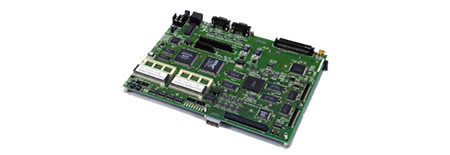
\includegraphics[width=0.7\hsize]{image200705/solutionengine.jpg}
  \end{center}
  \caption{Solution Engine}
 \end{minipage}
 \begin{minipage}{0.5\hsize}
  \begin{tabular}{|l|l|} \hline
   & Solution Engine \\ \hline
   CPU & SH7709 ( 133Mhz ) \\ \hline
   memory & 32MB\\ \hline
   Flash & 4MB \\ \hline 
   IDE  & PCMCIA slot \\ \hline
   Ethernet & stnic \\ \hline
  \end{tabular}
 \end{minipage}
\end{figure}

% CAT
\begin{figure}[htbp]
 \begin{minipage}{0.5\hsize}
  \begin{center}
   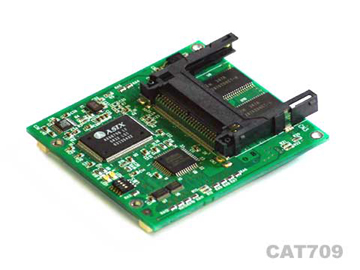
\includegraphics[width=0.6\hsize]{image200705/cat709.jpg}
  \end{center}
  \caption{CAT 709}
 \end{minipage}
 \begin{minipage}{0.5\hsize}
  \begin{tabular}{|l|l|} \hline
   & Solution Engine \\ \hline
   CPU & SH7709 ( 133Mhz ) \\ \hline
   memory & 32MB\\ \hline
   Flash & 8MB \\ \hline 
   IDE slot & CF Slot \\ \hline
   Ethernet & なし\\ \hline
  \end{tabular}
 \end{minipage}
\end{figure}

% Jornada 6xx
その他に Hewlett-Packard 社から販売されていた、Jornada6xx シリーズも使われていたとのこと。

%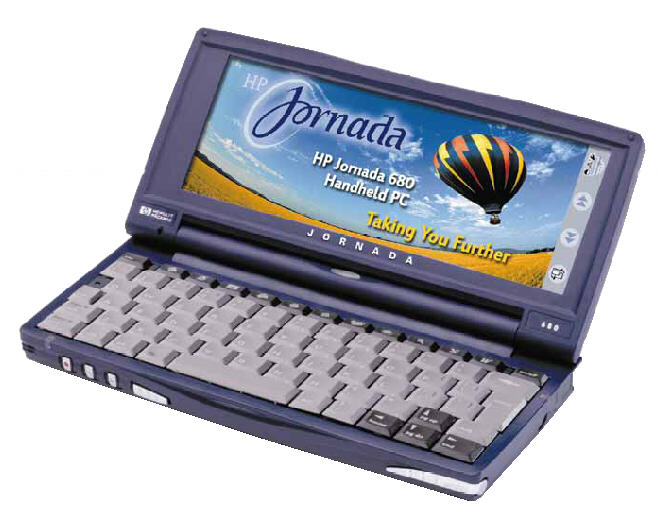
\includegraphics[width=0.2\hsize]{image200705/jornada680.jpg}

\subsubsection{第 1 次 SHブーム}

約2年前、SH を採用した NAS 、LANDISK / LANTANK  が I/Oデータさんから販売されました。
これらは I/O データさんに在籍しておられる、kinneko さん \footnote{http://d.hatena.ne.jp/kinneko/} および iohack project \url{http://iohack.sourceforge.net}
の元、開発が行われ Debian パッケージでシステムが構築されていました。
安値であり、自由に触ることができるということで、人気があり、各 Linux 雑誌でも取り扱われ、ブームを築きました。
これが 第 1 次 SH ブームです。

以下に LANDISK / LANTANK のスペックを示します。
\begin{figure}[htbp]
 \begin{minipage}{0.5\hsize}
  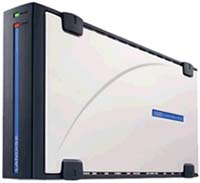
\includegraphics[width=0.6\hsize]{image200705/landisk00.jpg}
  \caption{LANDISK}
 \end{minipage}
 \begin{minipage}{0.5\hsize}
  \begin{tabular}{|l|l|} \hline
   & LANDISK \\ \hline
   CPU & SH7751R ( 266Mhz ) \\ \hline
   SDRAM & 64MB\\ \hline
   Flash & ROM \\ \hline
   IDE & UDMA133 PATA (ACARD ATP865)\\ \hline
   Ethernet & 10/100Base-T (RTL8139CL + EEPROM 93C46) \\ \hline
   USB & USB2.0 TypeA Conn x2 (NEC D720101GJ) \\ \hline
   値段 & 約35000円 \\ \hline 
 \end{tabular}
 \end{minipage}
\end{figure}


\begin{figure}[htbp]
 \begin{minipage}{0.5\hsize}
  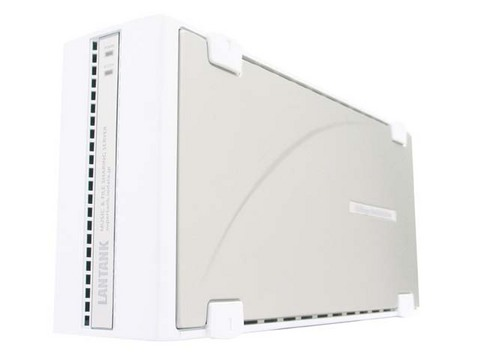
\includegraphics[width=0.9\hsize]{image200705/lantank00.jpg}
  \caption{LANTANK}
 \end{minipage}
 \begin{minipage}{0.5\hsize}
  \begin{tabular}{|l|l|} \hline
   & LANTANK \\ \hline
   CPU & SH7751R ( 266Mhz ) \\ \hline
   SDRAM & 64MB\\ \hline
   Flash & ROM \\ \hline
   IDE & UDMA133 PATA (ACARD ATP865) 2disk support  \\ \hline
   Ethernet & 10/100Base-T (RTL8139CL + EEPROM 93C46) \\ \hline
   USB & USB2.0 TypeA Conn x2 (NEC D720101GJ) \\ \hline
   値段 & 約19800円 \\ \hline
  \end{tabular}
 \end{minipage}
\end{figure}

しかし、SH の販売元であるルネサステクノロジはこのブームをうまく活用することができず、
そのまま消えていこうとしていたのでした。

\subsubsection{歴史は繰り返さないために}
終了してしまったように見えた、 SH の Debian への移植ですが、
私がパッケージを再ビルドし、再移植を行うことにしました。
理由としては、
\begin{itemize}
 \item SH で 容易に使用できるディストリビューションがない。
 
       gentoo でサポートされているが、ビルドが面倒。
 
 \item 仕事でも使えるようにしたい :)
       
	個人的理由。

 \item Debian User だから。
 
\end{itemize}

私は今回の移植では、以下のポリシーで作成することにしました。

\begin{itemize}
 \item Debian でサポートするアーキテクチャ

   SH4のみをサポートします。
   SH4A 等もすべてSH4として扱います。
   
 \item SH3 サポート
 
   SH3 と SH4 の大きな違いは FPU があるか、ないか です。
   SH3 は SH の Linux カーネルでサポートされた math-emu を使って、math をエミュレーションする方法を取ります。
   もちろん、math-emuを使うと、遅くなりますが、SH3 を採用した CPU がほとんど存在しないため、
   コストにはならないと考えています。
   
   他には、cache の違いもあるので、これをうまくトラップできる仕組みを入れる必要があります。
   
 \item big endian サポート
 
   big endian もサポートするすることも考えています。
   
\end{itemize} 

\subsection{現状}

\subsubsection{開発メンバー}
現在、基本的に開発を一人でやっていますが、以下の方々にサポートをしてもらっています。

\begin{itemize}

	\item 小島先生
		binutils SH メンテナ
		
		SH の分からないところは質問させていただいています。

	\item 武藤さん
	
		buildd の構築で相談に乗ってもらっています。

	\item kinnneko さん
	
		いろいろ手伝ってもらっています。

	\item gotom さん
	
		Debian glibc メンテナ.
		開発用のボードは渡したんだけど.....。

	\item 上川さん
	
		LANTANK買わせたんですが.....。
\end{itemize}

\newpage

\subsubsection{現在使用しているビルドマシン}

現在、ビルドに使用しているマシンは以下の通りです。

\begin{enumerate}

\item LANTANK x 3

\begin{figure}[htbp]
  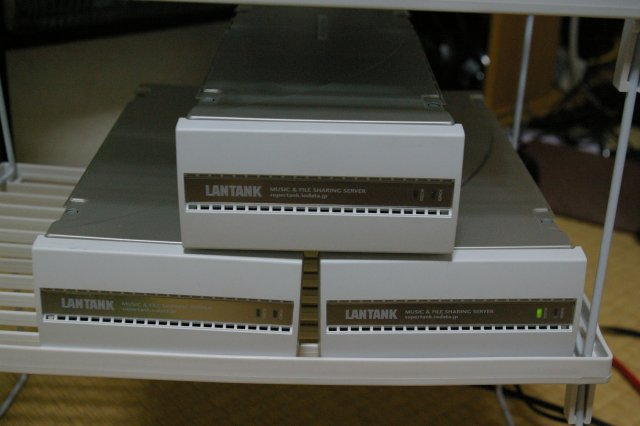
\includegraphics[width=0.8\hsize]{image200705/lantank01.jpg}
  \caption{LANTANK x 3} 
\end{figure}

\item RTS7751R2D

\begin{figure}[htbp]
 \begin{minipage}{0.5\hsize}
  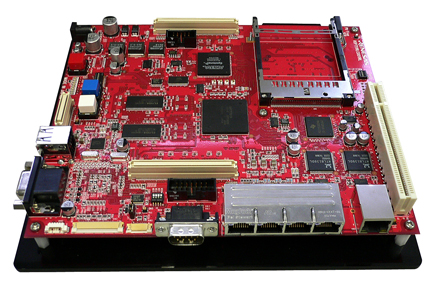
\includegraphics[width=0.9\hsize]{image200705/r2d.jpg}
  \caption{RTS7751R2D}
 \end{minipage}
 \begin{minipage}{0.5\hsize}
  \begin{tabular}{|l|l|} \hline
   & RTS7751R2D \\ \hline
   CPU & SH7751R ( 266Mhz ) \\ \hline
   SDRAM & 64MB\\ \hline
   Flash & ROM \\ \hline
   IDE & CF slot and  PCMCIA \\ \hline 
   Ethernet & 10/100Base-T (RTL8139CL + EEPROM 93C46) \\ \hline
   USB & SM501 USB1.1 (Silicom Motion) \\ \hline
  \end{tabular}
 \end{minipage}
\end{figure}

ルネサスソリューション様から提供していただきました。
\end{enumerate}

\subsubsection{パッケージ状況}

現在のパッケージ状況は以下の通りです。

\begin{itemize}
	\item SH4のみをサポート
	
		ビッグエンディアンのマシンを持っていないため。

	\item build-essential ビルド完了
	
		gcc-4.1.2 / binutils / glibc-2.5 

	\item sid debootstrap サポート
	
		debootstrap できるパッケージができています。

	\item SH4 buildd 稼働中
	
		公開はされていませんが、SH4 向けの buildd が稼動中です。
		今後、buildd.net \url{www.buildd.net} に登録する予定です。
		
\end{itemize}

これらの成果物を \url{http://www.nigauri.org/~iwamatsu/debian/debian-sh4/}で公開中です。

\subsection{今後の課題}

\begin{itemize}

\item Debian の正式なサポートアーキテクチャにする
\item buildd.net への登録
\item builddのメンテナンスが行える体制を作る

	共同メンテナを募集しています。
\item 回線の保持 

	buildd 用マシンネットワークの確保

\end{itemize}

\subsection{リンク}

\begin{itemize}
    \item SuperH \url{http://www.renesas.com}
    \item IRC \#debian-superh @ oftc.net
    \item ML  debian-superh@debian.org
    \item Debian Packages repository
	\url{http://www.nigauri.org/~iwamatsu/debian/debian-sh4/}

  \item iohack project
	\url{http://iohack.sourceforge.jp}

\end{itemize}


\dancersection{Debian の情報フロー}{上川}
\label{debianinfo}

\begin{minipage}{0.6\hsize}
 Debian etch を活用するためには、何をしたらよいですか?  今日のようにみん
 なあつまって議論すると、いろいろな新しい発見や情報が出てくるけど、それっ
 て普段みんなどうしているの?その疑問を追求するためにワークショップをして
 みました。

 まず建前から確認してみましょう。

 \begin{itemize}
  \item 基本はリリースノート
  \item BTS で生きた情報を得る
  \item debian-users メーリングリスト
 \end{itemize}

しかし実際の運用は少し違うこともあります。理由としては例えば次のようなも
 のがそれぞれあります。

\begin{itemize}
 \item リリースノート: 一度リリースされてしまうとそう簡単に項目が追加さ
       れる類のドキュメントではない。
 \item BTS: 英語なので日本では活用しているメンバーが限られる。また英
       語が問題とならなかったとしても、BTSの仕組みとして、情報がパッケー 
       ジ単位で管理されるため複合的に発生する問題は登録しにくい
\end{itemize}

現状の運用はどうかというと、ワークショップで出てきた話を総合すると、実際
は次のような流れになっているようですね。

 \begin{itemize}
  \item IRCでまずきく
  \item googleで検索 (blog とか スレッドテンプレで発見)
  \item 報告は blog に記述
  \item 2chで質問が出たりしたらblogを参照してスレッドテンプレに登録
 \end{itemize}
\end{minipage}
\begin{minipage}{0.4\hsize}
 \includegraphics[width=0.9\hsize]{image200705/problemcycle.eps}
\end{minipage}

では、現状を把握したところで、この仕組みのままで改善するか、違う仕組みを
考えるか、検討していけばよいはずです。続きはまた。

\cleartooddpage

\begin{minipage}[b]{0.2\hsize}
 \definecolor{titleback}{gray}{0.9}
 \colorbox{titleback}{\rotatebox{90}{\fontsize{80}{80} {\gt デビアン勉強会} }}
\end{minipage}
\begin{minipage}[b]{0.8\hsize}

\vspace*{15cm}
\hrule
\vspace{2mm}

\includegraphics[width=2cm]{image200502/openlogo-nd.eps}
\noindent \Large \bf Debian 勉強会資料\\ \\
\noindent \normalfont \debmtgyear{}年\debmtgmonth{}月\debmtgdate{}日 \hspace{5mm}  初版第1刷発行\\
\noindent \normalfont 東京エリア Debian 勉強会 (編集・印刷・発行)\\
\hrule
\end{minipage}

\end{document}
